%report.tex, Dan Richardson

%specify class of document
\documentclass[12pt, a4paper]{article}

%specify packages used 
\usepackage{microtype}		       %use package for minor typographical adjustments
\usepackage{graphicx} 		       %use package for diagram 
\usepackage{listings}                  %use package for c++ code in appendix
\usepackage{color}                     %use package for code listings
\usepackage[utf8]{inputenc}            %use package for colours in code
\usepackage{amsmath}                   %use package for various math symbols
\usepackage{amsfonts}                  %use package for number sets
\usepackage{bm}			       %use package for bolds in math mode
\usepackage{hyperref}                  %use package for hyperlinks
\usepackage{algpseudocode}             %use package for pseudocode
\usepackage{algorithm}                 %use package for pseudocode
\usepackage{fullpage}                  %use package for full page size
\usepackage{tikz}		       %use package for diagram drawings
\usepackage{caption}		       %use package for multiple figures
\usepackage{subcaption}                %use package for multiple figures
%\usepackage{url}                       %use package to display urls properly
%\usepackage{array}                     %use package for centering table contents

%set graphics path
\graphicspath{{/home/danmfr/p3t/laplace/images/}}

%define colours for code listings
\definecolor{codegreen}{rgb}{0,0.6,0}
\definecolor{codegray}{rgb}{0.5,0.5,0.5}
\definecolor{codepurple}{rgb}{0.58,0,0.82}
\definecolor{backcolour}{rgb}{0.95,0.95,0.92}

%define a style for the listings
\lstdefinestyle{mystyle}{
    backgroundcolor=\color{backcolour},
    commentstyle=\color{codegreen},
    keywordstyle=\color{magenta},
    numberstyle=\tiny\color{codegray},
    stringstyle=\color{codepurple},
    basicstyle=\footnotesize,
    breakatwhitespace=false,
    breaklines=true,
    captionpos=b,
    keepspaces=true,
    numbers=left,
    numbersep=5pt,
    showspaces=false,
    showstringspaces=false,
    showtabs=false,
    tabsize=2
}

%set style of listing to that defined above
\lstset{style=mystyle}

%use tikz library for shapes
\usetikzlibrary{shapes.geometric, arrows}

%define block styles in tikz
\tikzstyle{startstop} = [rectangle, rounded corners, minimum width=3cm, minimum height=1cm, text centered, draw=black, fill=red!30]
\tikzstyle{io} = [trapezium, trapezium left angle=70, trapezium right angle=110, minimum width=3cm, minimum height=1cm, text centered, draw=black, fill=blue!30]
\tikzstyle{process} = [rectangle, minimum width=3cm, minimum height=1cm, text centered, draw=black, fill=orange!30]
\tikzstyle{decision} = [diamond, minimum width=3cm, minimum height=1cm, text centered, draw=black, fill=green!30]
\tikzstyle{arrow} = [thick,->,>=stealth]

%set style of bibliography
\bibliographystyle{unsrt}

%set style of footnotes
\renewcommand{\thefootnote}{\roman{footnote}}

%define command shortcuts
\newcommand{\be}{\begin{equation}}
\newcommand{\ee}{\end{equation}}

%start of document
\begin{document}

%display title, my details and current date
\title{On the analytical and numerical solutions of Laplace's equation for different electrostatic configurations}
\author{S. Brown, F. Hayes, L. Heikkil{\"a}, D. Richardson\\
	School of Physics and Astronomy,\\
	University of Glasgow,\\
	Glasgow, United Kingdom}
\date{\today}
\maketitle

%start of abstract
\begin{abstract}

The behaviour of the electric field under the presence and influence of solid
conducting objects is modelled and studied. Finite difference methods, namely the
relaxation method, are employed to solve the Laplace equation numerically,
to find the approximate form of the electrostatic potential, and hence the electric
field, present in various electrostatic systems. We explicitly focus on two such
systems: the case of a long perfectly conducting cylinder centred between two infinite
planes at potential $+V$ and $-V$; and the case of a silicon detector---a system
composed of two silicon wafers with segmented doped implants at ground potential on one
side and a uniform doped implant, referred to as the backplane, on the other side, held
at a potential $+V$. We compare the analytical solution of the first system to its
approximate numerical solution, and study the convergence of the numerical method.

\end{abstract} % end of abstract

%start of introduction
\section{Introduction}
\subsection{Laplace's Equation}

Gauss' Law may used to express the relation between the \emph{divergence} of the
electric field, represented by \textbf{E}, and the \emph{charge density} $\rho$,
where $\epsilon_0$ is the \emph{permittivity of free space}:
%
\be
\nabla \cdot \bm{E} = \frac{\rho}{\epsilon_0}
\ee
%
Alternatively (c.f. the Divergence Theorem), it can be expressed in its
integral form, as:
%
\be
\oint \limits_S \bm{E} \cdot d\bm{A} = \frac{Q}{\epsilon_0}
\ee
%
where the integral is taken over a closed surface, $S$, and $Q$ is the enclosed charge.

In the absence of charge, as is the case outside a conductor, this reduces to the
statement the electric field is \emph{solenoidal}.

One can also relate the \emph{curl} of the electric field to the time
derivative of the magnetic field, denoted \textbf{B}:
%
\be
\nabla \times \bm{E} = - \frac{\partial \bm{B}}{\partial t}
\ee

If the magnetic field is constant, in other words unchanging with time, this equation
reduces to the statement that the electric field is \emph{irrotational}. A
consequence of irrotationality is that the electric field may then be written as
negative the gradient of some scalar potential, $\phi$ say. Mathematically:
%
\be
\bm{E} = -\nabla \phi
\ee
%
This scalar potential is called the \emph{electrostatic potential}.
One then has \emph{Laplace's equation}:
%
\be
\nabla^2 \phi = 0
\ee
%
where
$\nabla^2 \equiv \frac{\partial^2}{\partial x^2}+\frac{\partial^2}{\partial y^2}+\frac{\partial^2}{\partial z^2}$ 
is the \emph{Laplacian operator}\footnote{Specifically in Cartesian co-ordinates}.

This is a second-order partial differential equation that can be solved, given some
well-posed boundary conditions, to find the electrostatic potential and electric field
for some physical system.

\subsection{Finite Difference Schemes}

It is often the case that differential equations, such as the Laplace equation, cannot
be solved analytically, and their solution must be numerically approximated.

To numerically approximate the solution to a differential equation it is
necessary to approximate the derivative of a function. The usual method employed to
do this is finite differencing. This approximates the derivative by using explicit
differencing to step the function from one value to the next in small 
increments of some variable. The smaller the increment used, the more accurate
the approximation, but the longer and more computationally intensive the process.

Suppose one wishes to approximate the first derivative of a function $f(t)$, say,
with respect to the variable $t$. The simplest way to do this is to discretise the
derivative and write
%
\be
\frac{df}{dt} \approx \frac{f(t+\Delta t) - f(t)}{\Delta t}
\ee
%
where $f(t+\Delta t)$ and $f(t)$ are two values of $f$, evaluated at two points
a distance $\Delta t$ apart. This is known as the \emph{forward difference approximation}.

To approximate the second derivative of a function, one writes
%
\be
\frac{d^2 f}{dt^2} \approx \frac{f'(t) - f'(t-h)}{\Delta t} \\
= \frac{\frac{f(t +\Delta t) - f(t)}{\Delta t} - \frac{f(t) - f(t -\Delta t)}{\Delta t}}{\Delta t} \\
= \frac{f(t +\Delta t) - 2f(t) + f(t-\Delta t)}{\Delta t ^2}
\ee

\subsubsection{The Relaxation Method}

For our purposes, we wish to discretise the following equation:
% 
\be 
\frac{\partial^2 \phi}{\partial x^2}+\frac{\partial^2 \phi}{\partial y^2} = 0
\label{eq:laplace}
\ee 

One can define a region on which to discretise this equation, $\{(x,y)|0<x<L,0<y<D\}$,
and define a grid of points of spacial separation in $\Delta x$ in the $x$ direction,
and $\Delta y$ in the $y$ direction. We wish to find the value of $\phi$ at each point.

One can now approximate Equation~\ref{eq:laplace} as:
% 
\be
\frac{\phi_{j+1,k}-2\phi_{j,k}+\phi_{j-1,k}}{\Delta x^2} = - \frac{\phi_{j,k+1}-2\phi_{j,k}+\phi_{j,k-1}}{\Delta y^2}
\ee
%
where $j$ and $k$ index the $x$ and $y$ directions respectively.

If we use the same spacing $\Delta=\Delta x=\Delta y$ in both $x$ and $y$ directions this
reduces to:
%
\be
\phi_{j,k}= \frac{1}{4}(\phi_{j-1,k}+\phi_{j+1,k}+\phi_{j,k-1}+\phi_{j,k+1})
\label{eq:relax}
\ee
%
In other words the value of the potential at a specific point is the average
of the value of the potential at the four surrounding points. 

Suppose one has some initial guess of the value of $\phi$ at all points, $\phi_{j,k,0}$,
say. One evaluates Equation~\ref{eq:relax} at all points on the grid simultaneously and
generates a new better approximation for the potential, $\phi_{j,k,1}$. Iterating this
process $n$ times, one has
%
\be
\phi_{j,k,n+1}= \frac{1}{4}(\phi_{j-1,k,n}+\phi_{j+1,k,n}+\phi_{j,k-1,n}+\phi_{j,k+1,n})
\ee
%
This is known as \emph{Jacobi's iterative method}, and after each iteration the
approximation converges, or \emph{relaxes}, towards the correct solution. Hence, it is
also known as the \emph{relaxation method}.

\subsubsection{The Gauss-Seidel Method}

It is often unfeasible and computationally intensive to store the previous value of the
potential at each point, as in the Jacobi iterative method. An alternative method, known
as the \emph{Gauss-Seidel method}, exists where it is not neccessary to do this, and
instead the iterative algorithm is defined by
%
\be
\phi_{j,k,n+1}= \frac{1}{4}(\phi_{j-1,k,n+1}+\phi_{j+1,k,n}+\phi_{j,k-1,n-1}+\phi_{j,k+1,n})
\ee
%
where the previous points $\phi_{j-1,k}$ and $\phi_{j,k-1}$ have already been updated
by the algorithm as it loops through the grid.

It can be shown that this method actually converges faster than Jacobi's iterative
method, and it also has the added bonus of not requiring the previous value of the 
potential at each grid point to be stored.

\subsubsection{Successive Over-Relaxation}

Neither the Jacobi iterative method or the Gauss-Seidel method utilise the value
of the potential at the current point in the previous iteration, in our notation
$\phi_{j,k,n}$. It can be shown that using this point, defining a
\emph{relaxation parameter}, $1<s<2$, and defining an iterative algorithm as shown
%
\be
\phi_{j,k,n+1}= (1-s)\phi_{j,k,n}+\frac{s}{4}(\phi_{j-1,k,n+1}+\phi_{j+1,k,n}+\phi_{j,k-1,n-1}+\phi_{j,k+1,n})
\ee
%
results in a more convergent numerical method. This technique is known as
successive over-relaxation.

\subsubsection{Checkerboard (Red-Black) Updating}

%start of section
\section{System One}

Suppose one has a perfectly uniform electric field between two infinite planes
at potentials $V$ and $-V$, and they are a distance $2d$ apart. Suppose one then
places an infinitely long perfectly conducting cylinder, of radius $R$, into the centre
of the field, at ground potential, as in Figure~\ref{fig:sys one}. We wish to find the
resulting form of the electrostatic potential, and hence the electric field, surrounding
the cylinder.

\begin{figure}[h!]
\begin{center}
\begin{tikzpicture}
\draw (0,0) node[below] {$x = -d$} -- (0,6) node[above] {$\phi = V$}; 
\draw (10,0) node[below] {$x = d$} -- (10,6) node[above] {$\phi = -V$}; 
\draw (5,3) circle (1cm) node[below] {$\phi=0$};
\draw[dashed] (5,3) -- (5.6,3.8) node[pos=0.5,above left] {$R$};
\end{tikzpicture}
\end{center}
\caption{Cross-sectional diagram of System One}
\label{fig:sys one}
\end{figure}

\subsection{Analytic Solution}

First, one realises that the three-dimensional problem can be reduced entirely to two
dimensions due to the translation symmetry of the system along the length of the
cylinder. So, we consider a cross-section of the system and introduce a polar
co-ordinate system, with origin centred on the centre of the cylinder.

Laplace's equation in polar co-ordinates is: 
%
\be
\frac{\partial^2 \phi}{\partial r^2}+\frac{1}{r}\frac{\partial \phi}{\partial r}+\frac{1}{r^2}\frac{\partial^2 \phi}{\partial \theta^2}
= \frac{1}{r}\frac{\partial}{\partial r}(r \frac{\partial \phi}{\partial r}) + \frac{1}{r^2}\frac{\partial ^2 \phi}{\partial \theta^2}
= 0
\ee

We employ separation of variables and posit a solution of the form
$\phi = f(r)g(\theta)$ for two unknown functions $f$ and $g$. Upon substitution,
one finds that:
%
\be
\frac{r}{f(r)}\frac{d}{dr}(r \frac{df(r)}{dr}) =- \frac{1}{g(\theta)}\frac{d^2 g(\theta)}{d\theta^2}
\ee

Since this is true for arbitrary values of $r$ and $\theta$, it is constant, and
we---with some foreknowledge---set this equal to $k^2$, for some constant 
$k\in\mathbb{R}$.
This gives two second order ordinary differential equations:
%
\be
r\frac{d}{dr}(r \frac{df(r)}{dr}) = k^2 f(r) \qquad
\frac{d^2 g(\theta)}{d\theta^2}=-k^2 g(\theta)
\ee

For the case $k=0$, these equations have solutions
$f(r)=\alpha \ln(r) + \beta$ and $g(\theta) = \gamma \theta + \delta$.
For non-zero $k$, they have solutions
%
\be
f(r)=\alpha_k r^k + \beta_k r^{-k}
\qquad
g(\theta)= \gamma_k \sin(k\theta)+\delta_k \cos(k\theta)
\ee

With the physically reasonable requirement that $g(\theta)=g(\theta + 2\pi)$, we have
that $k$ is an integer. Hence, by the principle of superposition and the linearity of
differentiation, the general solution to the Laplace equation in polar co-ordinates is
a sum of these terms:
%
\be
\phi(r,\theta)
= f(r)g(\theta)
= (\alpha \ln(r) + \beta)(\gamma\theta + \delta) + \sum_{n=1}^{\infty}(\alpha_n r^n+\beta_n r^{-n})(\gamma_n \sin(n\theta) + \delta_n \cos(n\theta))
\ee

For a particular solution to the system considered here one must impose boundary
conditions, specifically we use \emph{Dirichlet boundary conditions}.

By considering the geometry of the system, we expect a solution that is symmetric
about $\theta=0$. This implies that $\gamma = 0$ and $\gamma_n=0$, $\forall n$ as
$\sin()$ is anti-symmetric about the origin (c.f. odd). Additionally, the potential
is finite as $r \rightarrow \infty$, implying that $\alpha$ and $\alpha_n$ are both
zero. We now have:
%
\be
\phi(r,\theta)=\beta + \sum_{n=1}^{\infty}(\frac{\beta_n}{r^n} \cos(n\theta))
\ee
%
where the $\beta$'s have absorbed other constants. In particular, as
$r \rightarrow \infty$, we require $\phi=-\frac{V}{d}x=-\frac{V}{d}r\cos(\theta)$.
Since the infinite sum vanishes at infinity, $\beta=-\frac{V}{d}r\cos(\theta)$.

We now have that
%
\be
\phi(r,\theta)=-\frac{V}{d}r\cos(\theta) + \sum_{n=1}^{\infty}(\frac{\beta_n}{r^n} \cos(n\theta))
              =(\frac{\beta_1}{r}-\frac{V}{d}r)\cos(\theta) + \sum_{n=2}^{\infty}(\frac{\beta_n}{r^n} \cos(n\theta))
\ee

We require that the potential is zero on the surface of the cylinder,
$\phi(R,\theta)=0$, so that $\beta_1=\frac{VR^2}{d}$ and $\beta_{n \geq 2}=0$

Thus, the final form for the electrostatic potential is
%
\be
\phi(x,y)=
\begin{cases} \qquad 0, & \quad r \leq a \\
\frac{V}{d}(\frac{R^2}{r}-r)\cos(\theta), & \quad r > a
\end{cases}
\ee
%
a graph of which is shown in Figure~\ref{fig:analytic}.

\begin{figure}
\begin{center}
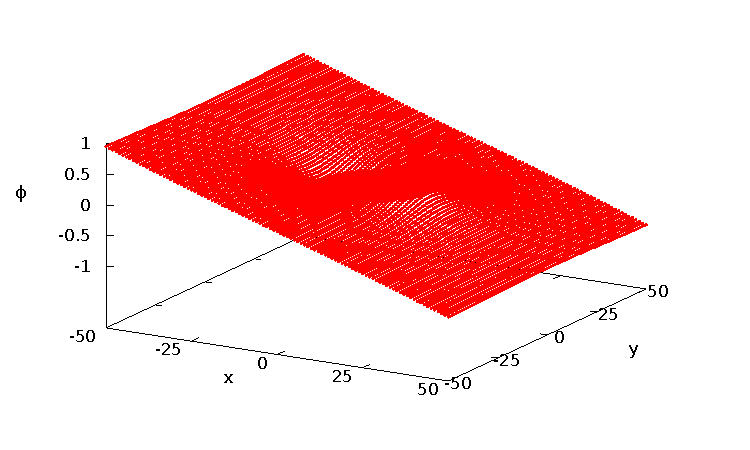
\includegraphics{analytic.pdf}
\caption{Analytic solution with $V=1$, $R=15$ on $100\times100$ grid}
\label{fig:analytic}
\end{center}
\end{figure}

\subsection{Numerical Solution}

To numerically approximate the electrostatic potential for System 1 via the 
relaxation method the following rudimentary algorithm was developed.

\begin{algorithm}
\begin{algorithmic}[1]
\Procedure{The Relaxation Method}{}
\State declare variables:
\State $V \gets$ potential on plates
\State $\delta \gets$ position step-size
\State $d \gets$ distance between plates
\State $h \gets$ height of plates
\State $r \gets$ radius of cylinder
\State $its \gets$ number of iterations
\State $nx \gets \frac{d}{\delta}$ 
\State $ny \gets \frac{h}{\delta}$ 
\State specify boundary potentials:
\For {$j=1$ to $ny$}
   \State $u_{j, 1} = +V$
   \State $u_{j, nx} = -V$
\EndFor
\For {$k=1$ to $nx$}
   \State $u_{1, k} \gets V-\frac{2Vj}{nx}$
   \State $u_{ny, k} \gets V-\frac{2Vj}{nx}$
\EndFor
\State find solution:
\For {$i=1$ to $its$}
   \For {$j=2$ to $ny-1$}
      \For {$k=2$ to $nx-1$}
         \If {$(j \delta-\frac{1}{2} d)^2+(k \delta-\frac{1}{2} h)^2<r^2$}
            \State $u_{j, k} \gets 0$
         \Else
            \State $u_{j,k} \gets \frac{1}{4}(u_{j-1,k}+u_{j+1,k}+u_{j,k-1}+u_{j,k+1})$
         \EndIf
      \EndFor
   \EndFor
\EndFor
\State find electric field:
\For {$j=1$ to $ny-1$}
   \For {$k=1$ to $nx-1$}
      \State $(Ex)_{j, k} \gets -\left(u_{j,k+1}-u_{j,k}\right)/\delta$
      \State $(Ey)_{j,k} \gets -\left(u_{j+1,1}-u_{j,k}\right)/\delta$
   \EndFor
\EndFor
\State plot potential and field
\EndProcedure
\end{algorithmic}
\end{algorithm}

Figure~\ref{fig:numerical} shows the numerical approximation to the potential,
and Figure~\ref{fig:field} shows the electric field around the cylinder.

\begin{figure}
\centering
\begin{subfigure}[b]{0.7\textwidth}
	\includegraphics[width=\textwidth]{potentialA.pdf}
	\caption{electrostatic potential}
	\label{fig:numerical}
\end{subfigure}

\begin{subfigure}[b]{0.7\textwidth}
	\includegraphics[width=\textwidth]{fieldA.pdf}
	\caption{electric field}
	\label{fig:field}
\end{subfigure}
\caption{Numerical approximations for electstatic potential and electric field with
$V=1$, $R=15$ on $100\times100$ grid for $10000$ iterations}
\end{figure}

\subsection{Comparison of Analytical and Numerical Solution}

%start of section
\section{System Two}

The second system considered was a silicon detector---a system consisting of two
silicon wafers, one segmented with doped implants at ground potential and the other,
referred to as the backplane, uniformly doped, held at a potential $+V$, as shown
in Figure~\ref{fig:sys two}.

\begin{figure}[h!]
\begin{center}
\begin{tikzpicture}
\draw (0,0) -- (12,0) node[right] {$\phi = V$}; 
\draw (0,5) -- (12,5) node[pos=0.25, above] {GND} node[pos=0.5, above] {GND} node[pos=0.75,above] {GND}; 
\draw (2.5,5) rectangle (3.5,4.75);
\draw (5.5,5) rectangle (6.5,4.75);
\draw (8.5,5) rectangle (9.5,4.75);
\end{tikzpicture}
\end{center}
\caption{Cross-sectional diagram of System Two}
\label{fig:sys two}
\end{figure}

\subsection{Numerical Solution}

%start of section
\section{Other Electrostatic Systems}

We developed a general software package in C++ to solve and plot the potential and
electric field for an arbitrary electrostatic system. It accepts input of a coloured
bitmap, where the colours represent different potentials, and returns plots of the
resultant electrostatic potential and electric field.

Figure~\ref{fig:flowchart} shows a flowchart representing the algorithm employed.

\begin{figure}[htbp!]
\begin{center}
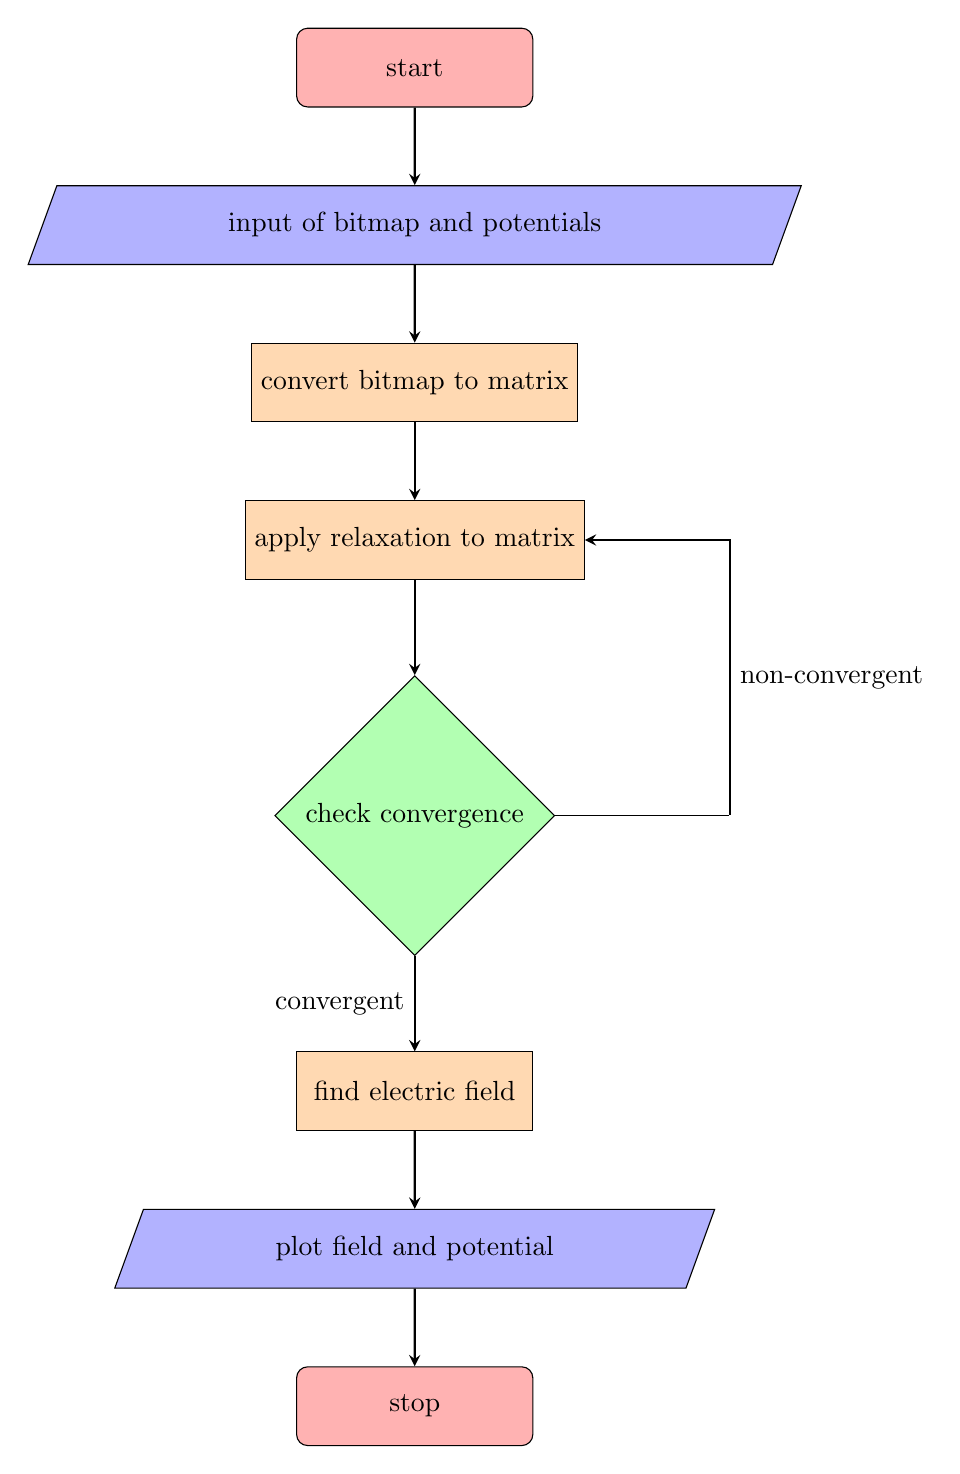
\begin{tikzpicture}[node distance=2cm]

\node (start) [startstop] {start};
\node (in1) [io, below of=start] {input of bitmap and potentials};
\node (pro1) [process, below of=in1] {convert bitmap to matrix};
\node (pro2) [process, below of=pro1] {apply relaxation to matrix};
\node (dec1) [decision, below of=pro2, yshift=-1.5cm] {check convergence};
\node (inv) [inner sep=0, minimum size=0, right of=dec1, xshift=2cm] {}; % invisible node
\node (pro3) [process, below of=dec1, yshift=-1.5cm] {find electric field};
\node (out1) [io, below of=pro3] {plot field and potential};
\node (stop) [startstop, below of=out1] {stop};

\draw [arrow] (start) -- (in1);
\draw [arrow] (in1) -- (pro1);
\draw [arrow] (pro1) -- (pro2);
\draw [arrow] (pro2) -- (dec1);
\draw [arrow] (dec1) -- node[left] {convergent} (pro3);
\draw (dec1) -- (inv);
\draw [arrow] (inv) |- node[pos=0.25, right] {non-convergent} (pro2);
\draw [arrow] (pro3) -- (out1);
\draw [arrow] (out1) -- (stop);

\end{tikzpicture}
\end{center}
\caption{Flowchart of steps in software package}
\label{fig:flowchart}
\end{figure}

\subsection{Bitmaps, Boolean Masks and Convergence}
\subsection{Timing and CPU usage}

%start of section
\section{Conclusion}

\subsection{Further Work}

%include BibTex bibliography
\bibliography{report}

%start of appendix
\appendix
\section{Appendices}

\end{document} %end of document
